%%%%% Kompendium -- Wellen und Optik %%%%%
%% Optik %%


%Some sample text to be displayed above the first subsection

%\subsection{Prinzip}

%Ein Zyklotron besteht aus Zwei hohlen, halbzylindrischen und Duanden an denen eine Spannung mit unterschiedlichem Vorzeichen anliegt, und darüber bzw. darunter liegende Magneten, die ein homogenes Magnetfeld erzeugen. Zudem gibt es einen Einlass und einen Auslass für Teilchen.

%\begin{wrapfigure}{r}{0.4\textwidth} \label{Zyklo}
%
%	\vspace{-10pt}
%	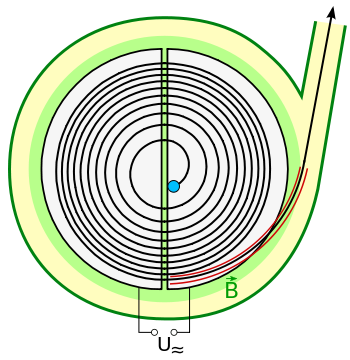
\includegraphics[width=0.35\textwidth]{Zyklotron_Prinzipskizze02.png}
%	\vspace{-13pt}
%	\caption{Prinzipskizze eines Zyklotrons}
%	\vspace{-5pt}	
%	
%\end{wrapfigure}

%\subsubsection{Anwendung}

% Some Formula:

%\begin{equation}
%	x= \frac{y \cdot 13 \pi z}
%			{\cos \alpha}
%\end{equation}

%%%%%%%%%%%%%%%%%%%%%%%
% Eigentlicher Beginn %
%%%%%%%%%%%%%%%%%%%%%%%


\subsection{Brechung von Licht}

Wenn Licht von einem Medium in ein anderes übergeht wird es gebrochen, das heißt, es seine Richtung ändert sich. Die Brechung ist hauptsächlich vom Quotienten der Lichtgeschwindigkeiten in den Materialien abhängig, jedoch spielt auch die Wellenlänge eine Rolle, da kurzwelliges Licht etwas stärker gebrochen wird als langwelliges.

Brechung ist an folgendem Diagramm recht einfach mit dem Huygens'schen Prinzip (\referenz{subsec:ausbreitung}) zu erklären: \footnote{„Refraction - Huygens-Fresnel principle“ von Arne Nordmann (norro) - Own illustration, based on Image:Wellen-Brechung.png and Image:Huygens\_brechung.png. Lizenziert unter CC BY-SA 3.0 über Wikimedia Commons - \url{https://commons.wikimedia.org/wiki/File:Refraction\_-\_Huygens-Fresnel\_principle.svg}}

\begin{figure}[h!]
	\center
	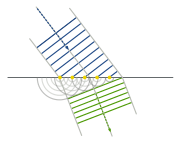
\includegraphics[width=0.5\textwidth]{brechung}
	\caption{Brechung mit dem Huygens'schen Prinzip}
\end{figure}

Die Abbildung zeigt den Übergang eines schmalen, monochromatischen (nur eine Farbe/Wellenlänge) Lichtbündels in ein Material mit einer niedrigeren Lichtgeschwindigkeit. Das Lichtbündel ist faktisch eine phasengleiche Welle, die Schräg auf der Übergangsfläche auftrifft. So löst ein Wellenberg auf der linken Seite früher Elementarwellen aus als auf der rechten Seite. Da die Elementarwellen im neuen Medium langsamer sind als im alten wird der Lichtstrahl zum Lot hin gebrochen.

\subsubsection{Mathematisierung}

	Man denke sich nun ein senkrechtes Lot an die Kante des Materialübergangs. Die Winkel $\alpha$ sein der Winkel des Stahls im ersten Medium zum Lot und $\beta$ der Winkel des Strahls im neuen Medium zum Lot hin. Dann gilt folgendes:
	
	\begin{equation}
		\frac{sin{(\alpha)}}{sin{(\beta)}} = \frac{c_1}{c_2}
	\end{equation}
	
	Unter Berücksichtung der verschieden Brechungen von verschiedenen Wellenlängen muss eine neue Größe eingeführt werden, die Brechzahl $n$. Folgendes ergibt sich:
	
	\begin{equation} \label{eq:brechungsgesetz}
		\frac{sin{(\alpha)}}{sin{(\beta)}} = \frac{n_2}{n_1}
	\end{equation}






